\section{Method}
\subsection{The Bluff Body}
\label{sec:bluffBody}
In order to maintain a cylinder-like appearance, one of the most common bluff bodies investigated \parencite[475]{rocchi2002_vortex}, this investigation used bluff bodies which have a rectangular “tail”. This results in each bluff body having an overall length $\ell$ in both streamwise and transverse directions \textemdash\ like a cylinder. The characteristic length $L$ of each bluff body is therefore equal to the overall length $\ell$. Bluff bodies with streamwise faces $n$ ranging from $2$ to $12$ were investigated. The lengths of the $n$ faces within the bluff body $n$ were homogeneous. A square bluff body ($n=1$) was excluded due to its fundamentally different flow interaction attributed to the lack of multiple streamwise faces. 
\begin{figure}[H]
	\begin{center}
		\begin{tikzpicture}[line join=round, line cap=round, scale=0.7]
			\node at (9,6) {\large \textbf{Inlet}};
			\draw[->, line width=1pt] (3,5) -- (3, 4);
			\draw[->, line width=1pt] (6,5) -- (6, 4);
			\draw[->, line width=1pt] (9,5) -- (9, 4);
			\draw[->, line width=1pt] (12,5) -- (12, 4);
			\draw[->, line width=1pt] (15,5) -- (15, 4);
			
			\draw (-1,0.8) -- (-1,2.8);     
			\draw (-1,2.8) -- (-0.7,2.8);   
			\draw (-1,0.8) -- (-0.7,0.8);
			
			\node[anchor=east] at (-1, 1.8) {$n$ faces};
			
			\draw (-1,-1.2) -- (-1,0.8);     
			\draw (-1,0.8) -- (-0.7,0.8);   
			\draw (-1,-1.2) -- (-0.7,-1.2);
			
			\node[anchor=east, align=right] at (-1, -0.2) {Rectangular \\[-0.7em] “tail”};
			
			
			\begin{scope}[yshift=-35] 
				% Base shape dimensions
				\def\W{4}   % width of the base
				\def\H{2}   % height of the base
				\def\R{2}   % roof "radius"
				
				\draw[<->] (9, 4) -- (9, 0);
				\node[anchor=west] at (9, 3) {$\ell$};
				
				\draw[<->] (7, 2) -- (11, 2);
				\node[anchor=north] at (8, 2) {$\ell$};
				
				% --- LEFT: 2-sided roof (n=2) ---
				\coordinate (A) at (0,0);
				\coordinate (B) at (\W,0);
				\draw (A) -- (B) -- (\W,\H)
				-- (\W/2,\H+\R) -- (0,\H) -- cycle;
				\node[below=8pt of $(A)!0.5!(B)$] {$n = 2$};
				
				% --- MIDDLE: 6-sided roof (n=6) ---
				\begin{scope}[xshift=7cm]
					\coordinate (A) at (0,0);
					\coordinate (B) at (\W,0);
					\draw (A) -- (B);
					\draw (A) -- (0,\H);
					\draw (B) -- (\W,\H);
					
					\foreach \k [evaluate=\k as \ang using {180 - 30*\k}] in {0,...,6}{
						\coordinate (m\k) at ({\W/2 + \R*cos(\ang)},
						{\H   + \R*sin(\ang)});
					}
					\draw (0,\H) -- (m0);
					\foreach \k in {0,...,5}{
						\pgfmathtruncatemacro\next{\k+1}
						\draw (m\k) -- (m\next);
					}
					\draw (m6) -- (\W,\H);
					\node[below=8pt of $(A)!0.5!(B)$] {$n = 6$};
				\end{scope}
				
				% --- RIGHT: 12-sided roof (n=12) ---
				\begin{scope}[xshift=14cm]
					\coordinate (A) at (0,0);
					\coordinate (B) at (\W,0);
					\draw (A) -- (B);
					\draw (A) -- (0,\H);
					\draw (B) -- (\W,\H);
					
					\foreach \k [evaluate=\k as \ang using {180 - 15*\k}] in {0,...,12}{
						\coordinate (r\k) at ({\W/2 + \R*cos(\ang)},
						{\H   + \R*sin(\ang)});
					}
					\draw (0,\H) -- (r0);
					\foreach \k in {0,...,11}{
						\pgfmathtruncatemacro\next{\k+1}
						\draw (r\k) -- (r\next);
					}
					\draw (r12) -- (\W,\H);
					\node[below=8pt of $(A)!0.5!(B)$] {$n = 12$};
				\end{scope}
			\end{scope}
		\end{tikzpicture}
	\end{center}
	\caption{Examples of bluff bodies}
	\label{fig:bluffBodies}
\end{figure}
\subsection{The Theoretical Investigation}
\subsubsection{Ansys Workbench}
\label{sec:ansysWorkbench}
The geometry and mesh preparation for the simulation was conducted using Ansys Workbench \parencite{noauthor_ansys_nodate}. The dimensions of the fluid domain are based on Figure \ref{fig:fluidDomain} where $\ell$ is the overall length of the bluff body.

\newlength\unitL
\setlength\unitL{0.2cm}

\begin{figure}[H]
	
	\begin{center}
		\begin{tikzpicture}[x=\unitL, y=\unitL, >=stealth, line width=1pt]
			
			% === Outer domain ===
			\draw (0,0) rectangle (63,50);
			
			% === Bluff Body ===
			\draw (22, 25) -- (23, 24);
			\draw (23, 24) -- (24, 24);
			\draw (24, 24) -- (24, 26);
			\draw (23, 26) -- (24, 26);
			\draw (22, 25) -- (23, 26);
			
			\draw[<->] (25, 24) -- (25, 26);
			\node at (27, 25) {$\ell$};  
			
			\draw[<->] (22, 23) -- (24, 23);
			\node at (23, 21) {$\ell$};  
			
			% === Velocity inlet arrows (spaced + farther from wall) ===
			\foreach \y in {12,20,28,36}
			\draw[->] (-5,\y) -- (-1,\y);  % stop at x=0.3 to add gap
			
			% === Velocity inlet label (more horizontal distance) ===
			\node[rotate=90] at (-7,25) {\large \textbf{Velocity Inlet}};
			
			% === Pressure outlet ===
			\draw[<->] (65.5,0) -- (65.5,50);
			\node[rotate=90] at (72,25) {\large \textbf{Pressure Outlet}};
			\node[rotate=90] at (68,25) {$25\,\ell$};
			
			% === Bottom dimensions (same horizontal alignment) ===
			\draw (23,0) -- (23,-0.8);  % tick at square center
			
			\draw[<->] (0,-3) -- (23,-3);  % from inlet to square center
			\node at (11.5,-5.1) {$11.5\,\ell$};
			
			\draw[<->] (23,-3) -- (63,-3); % from square center to outlet
			\node at (43,-5.1) {$20\,\ell$};
			
		\end{tikzpicture}
	\end{center}
	\caption{The fluid domain with dimensions. Example with bluff body $n = 2$. Inspired by \textcite{comflics_openfoam_2014}}
	\label{fig:fluidDomain}
\end{figure}

Given the computational limitations of the computer the simulation was conducted on, an overall length $\ell$ of $1\times{10}^{-3}\,m$ was chosen \textemdash\ therefore $L = 1\times{10}^{-3}\,m$. 

In order to create the mesh necessary for the simulation, the \textit{All Triangles Method} was utilized. A global unit size of $2.25\times{10}^{-3}\,m$ was applied to the fluid domain to ensure a computationally inexpensive resolution in regions of negligible interest. Conversely, near the edge of the bluff body, a significantly smaller unit size of $2.0\times{10}^{-5}\,m$ was used, constituting an accurate depiction of the interaction between the fluid flow and the bluff body \parencite{ansys_learning_best_2023}. Furthermore, eight inflation layers were employed in order to precisely capture the gradients associated with boundary layer formation at the edges of the bluff body \parencite{fluid_mechanics_101_cfd_2021}. Moreover, a body of influence (BOI) with a sizing of $2.0\times{10}^{-4}\,m$ was used \textemdash\ positioned as shown in Figure \ref{fig:fluidDomainWithBOI} \textemdash\ refining the mesh around the bluff body and also in the wake region (where the vortex shedding occurs), constituting for a more exact simulation.  

\begin{figure}[H]
	
	\begin{center}
		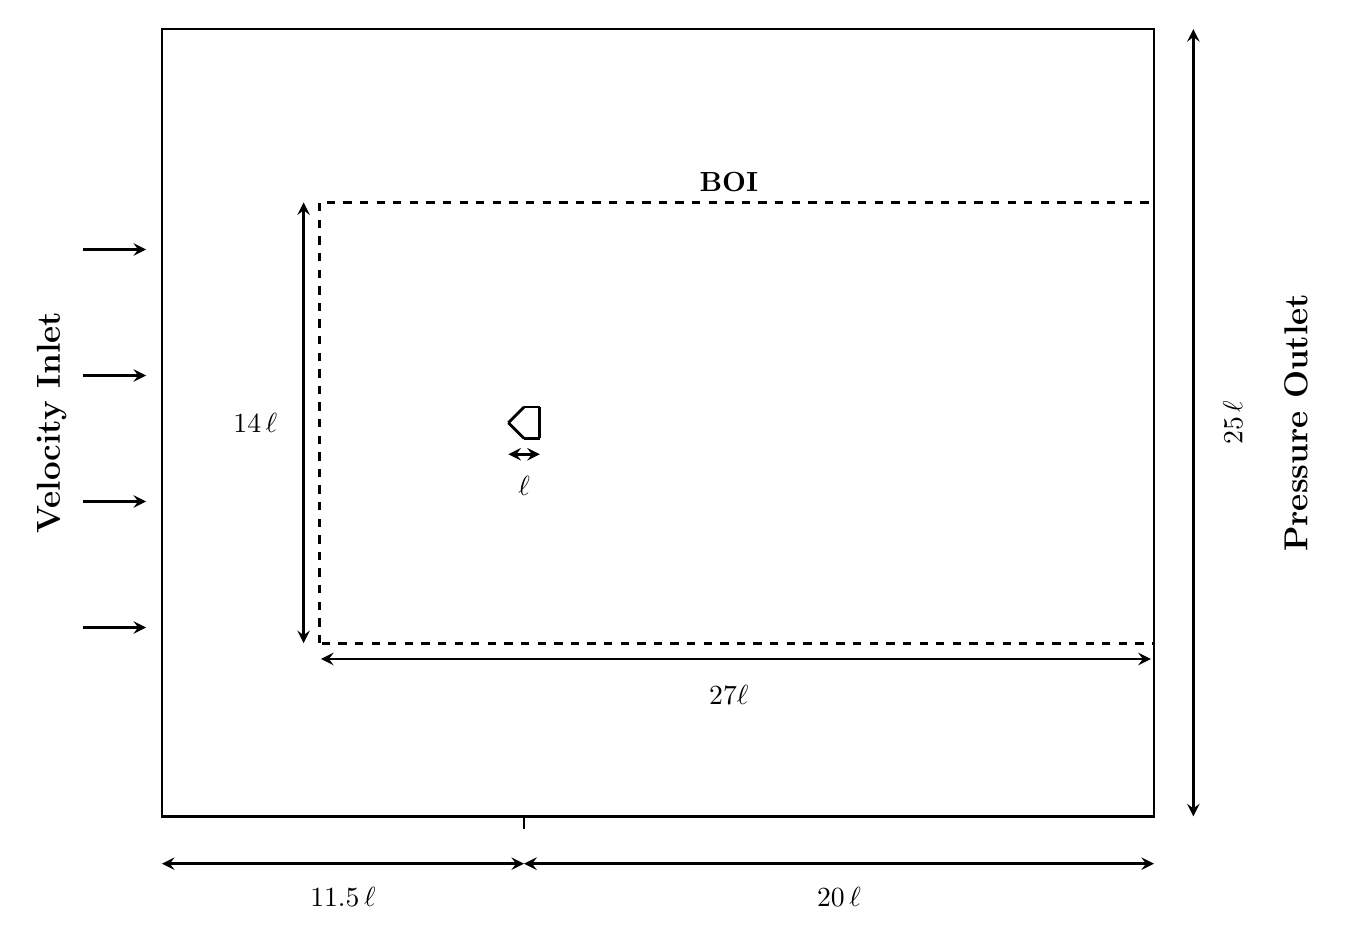
\begin{tikzpicture}[x=\unitL, y=\unitL, >=stealth, line width=1pt]
			
			% === Outer domain ===
			\draw (0,0) rectangle (63,50);
			
			% === BOI rectangle ===
			\draw[dashed] (10,11) rectangle (63,39);  % Body of Influence
			\node[anchor=south] at (36,39) {\textbf{BOI}};
			
			
			\draw[<->] (10.1,10) -- (62.8, 10);
			\node [anchor=north] at (36, 9) {$27 \ell$};
			
			\draw[<->] (9,11) -- (9,39);
			\node[anchor=east] at (8,25) {$14\,\ell$};
			
			% === Bluff Body ===
			\draw (22, 25) -- (23, 24);
			\draw (23, 24) -- (24, 24);
			\draw (24, 24) -- (24, 26);
			\draw (23, 26) -- (24, 26);
			\draw (22, 25) -- (23, 26);
			
			\draw[<->] (22, 23) -- (24, 23);
			\node at (23, 21) {$\ell$};  
			
			% === Velocity inlet arrows (spaced + farther from wall) ===
			\foreach \y in {12,20,28,36}
			\draw[->] (-5,\y) -- (-1,\y);  % stop at x=0.3 to add gap
			
			% === Velocity inlet label (more horizontal distance) ===
			\node[rotate=90] at (-7,25) {\large \textbf{Velocity Inlet}};
			
			% === Pressure outlet ===
			\draw[<->] (65.5,0) -- (65.5,50);
			\node[rotate=90] at (72,25) {\large \textbf{Pressure Outlet}};
			\node[rotate=90] at (68,25) {$25\,\ell$};
			
			% === Bottom dimensions (same horizontal alignment) ===
			\draw (23,0) -- (23,-0.8);  % tick at square center
			
			\draw[<->] (0,-3) -- (23,-3);  % from inlet to square center
			\node at (11.5,-5.1) {$11.5\,\ell$};
			
			\draw[<->] (23,-3) -- (63,-3); % from square center to outlet
			\node at (43,-5.1) {$20\,\ell$};
			
		\end{tikzpicture}
	\end{center}
	\caption{The fluid domain with dimensions  and the BOI. Example with bluff body $n = 2$. Inspired by \textcite{comflics_openfoam_2014}}
	\label{fig:fluidDomainWithBOI}
\end{figure}

\begin{figure}[H]
	\centering
	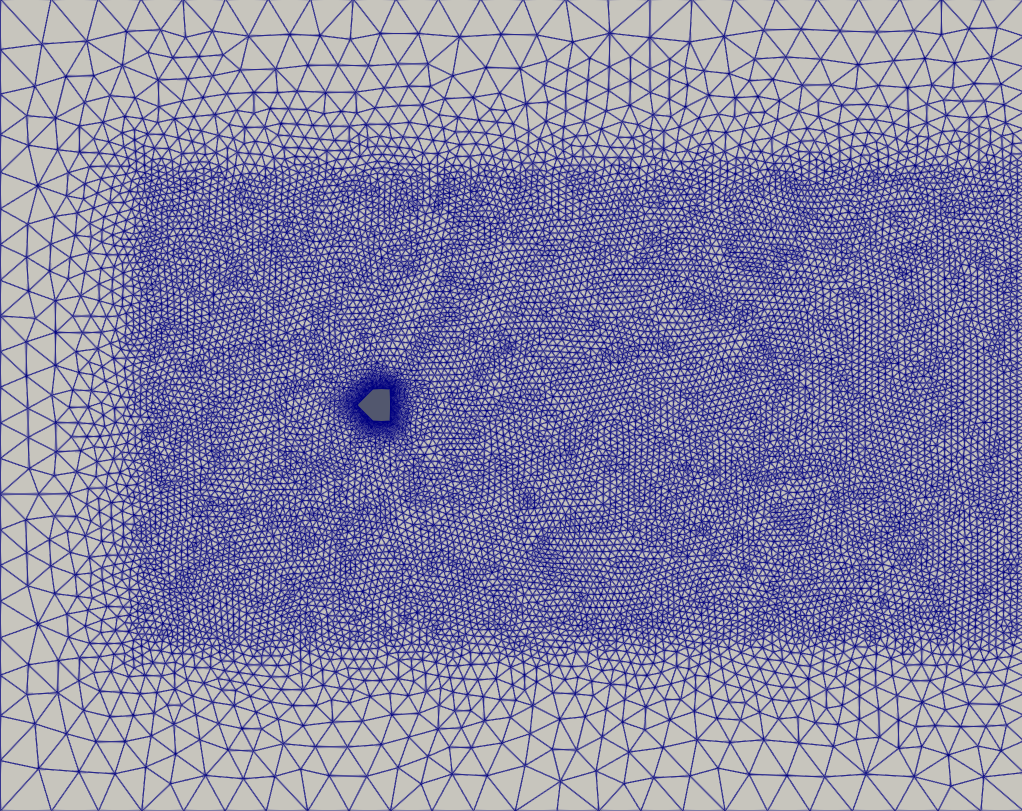
\includegraphics[width=\textwidth]{images/2FaceMesh}
	\caption{Example of mesh of fluid domain with bluff body $n = 2$. Visualized in ParaView}
	\label{fig:2FaceMesh}
\end{figure}

\subsubsection{The OpenFOAM Simulation}
\label{sec:openFoam}
The theoretical part of this EE was conducted using the open-source CFD software package OpenFOAM \parencite{noauthor_openfoam_2024} in Windows Subsystem for Linux (WSL) \parencite{noauthor_windows_nodate}. Among the numerous solvers OpenFOAM provides, pimpleFOAM is a transient, pressure-based solver for incompressible, single-phase flows \parencite{noauthor_pimplefoam_nodate}. It facilitates robust handling of transient simulations with larger time steps, allowing for improved computational performance. Moreover, its ability to model both laminar and turbulent flow ensures flow conditions are accurately reflected and given that the fluctuations of lift force in laminar flow are sinusoidal, one can verify the flow is laminar. Utilizing reporting functions, one can extract the lift coefficient $C_{L}$, which shows the fluctuations in the lift force acting on the bluff body.
\subsubsection{Simulation Settings}
To adhere to the scope of this essay, the simulation setup was adapted from a case study provided in the Udemy course \textit{OpenFOAM for Absolute Beginners} by \textcite{jayaraj2024openfoam}. The tutorial case \textit{3vortexShedding}, discussed in lecture eight, served as a structural template and was modified to align with the specific requirements of this investigation.

\vspace{1em}

\begin{figure}[H]
	\centering
	\begin{forest}
		for tree={
			font=\ttfamily,
			grow=east,
			child anchor=west,
			parent anchor=east,
			anchor=west,
			edge={draw,-stealth},
			inner sep=2pt,
			l sep=50pt,
			s sep=20pt
		}
		[case/
		[0/
		[\textcolor{blue}{U}]
		[p]
		[nuTilda]
		[nut]
		]
		[constant/
		[turbulenceProperties]
		[\textcolor{blue}{transportProperties}]
		[g]
		[\textcolor{green}{polyMesh/}
		[\textcolor{green}{pointZones}]
		[\textcolor{green}{points}]
		[\textcolor{green}{owner}]
		[\textcolor{green}{neighbor}]
		[\textcolor{green}{faceZones}]
		[\textcolor{green}{faces}]
		[\textcolor{green}{cellZones}]
		[\textcolor{green}{boundary}]
		]
		]
		[system/
		[fvSolution]
		[fvSchemes]
		[\textcolor{green}{forceCoeffs}]
		[\textcolor{blue}{decomposeParDict}]
		[\textcolor{blue}{controlDict}]
		]
		[\textcolor{blue}{para.foam}]
		[\textcolor{blue}{mesh.msh}]
		]
	\end{forest}
	\caption{Overview of the simulation directory structure. Modified files are highlighted blue. Created files and folders are highlighted green }
\end{figure}


\begin{table}[H]
	\centering
	\makebox[\linewidth][c]{
		\begin{tabularx}{1.2\textwidth}{|p{3cm}|p{3.3cm}|p{2.8cm}|p{3cm}|X|}
			\hline
			\textbf{File} & \textbf{Parameter} & \textbf{Original} & \textbf{Modified} & \textbf{Justification} \\
			\hline
			\verb*|mesh.msh|, \verb*|para.foam|, 
			\begin{tabular}[t]{@{}l@{}}
				\verb|polyMesh/|\\[-0.3em]
				\small\hspace{1.5em}\verb|boundary| \\[-0.3em]
				\small\hspace{1.5em}\verb|cellZones| \\[-0.3em]
				\small\hspace{1.5em}\verb|faces| \\[-0.3em]
				\small\hspace{1.5em}\verb|faceZones| \\[-0.3em]
				\small\hspace{1.5em}\verb|neighbor| \\[-0.3em]
				\small\hspace{1.5em}\verb|owner| \\[-0.3em]
				\small\hspace{1.5em}\verb|points| \\[-0.3em]
				\small\hspace{1.5em}\verb|pointsZones|
			\end{tabular} 
			
			& \textemdash & \verb*|mesh.msh| defines, \verb*|polyMesh/| contains and \verb*|para.foam| visualizes the mesh of fluid domain of tutorial case & \verb*|mesh.msh| defines, \verb*|polyMesh/| contains and \verb*|para.foam| visualizes the mesh of fluid domain with dimensions given in \Cref{sec:ansysWorkbench} & The fluid domain was adjusted to conform with the computational limits discussed in \Cref{sec:ansysWorkbench}, while achieving the Reynolds number required for this investigation\\
			\hline
			\verb*|controlDict| & \verb*|deltaT| & 0.0002 & 0.00001 &
			Decreased in order to achieve a greater accuracy \parencite[289]{versteeg2007} while ensuring numerical stability \parencite{caminha_cfl_2017}. 
			\\
			
			\rule{0pt}{5ex} & \verb*|functions| & \verb*|none| &
			\begin{tabular}[t]{@{}l@{}}
				\verb|#include| \\[-0.3em]
				\verb*|"forceCoeffs"|
			\end{tabular} &
			Reporting function, defined in \verb*|forceCoeffs|, included in order to extract the lift coefficient $C_L$ \parencite{codeynamics_prism_2024}
			\\ 
			
			\rule{0pt}{5ex} & {\small\verb*|adjustTimeStep|} & \verb*|yes| & \verb*|no| &
			Removed as the simulation demonstrated stable behavior with the adjusted \verb*|deltaT| \parencite{jayaraj2024openfoam}
			\\ 
			
			\hline
			
			
		\end{tabularx}
	}
	\caption{Overview of the changes made to the simulation template.}
	\label{tab:simulation_change1}
\end{table}

\begin{table}[H]
	\centering
	\renewcommand{\arraystretch}{1.3}
	\makebox[\linewidth][c]{
		\begin{tabularx}{1.2\textwidth}{|p{3cm}|p{3.3cm}|p{2.8cm}|p{3cm}|X|}
			\hline
			\textbf{File} & \textbf{Parameter} & \textbf{Original} & \textbf{Modified} & \textbf{Justification} \\
			\hline
			
			{\footnotesize\verb*|decomposeParDict|} & {\footnotesize\verb*|numberOfSubdomains|} & 8 & 6 & The simulations were performed on a system with \verb*|6| processing cores \parencite{jayaraj2024openfoam} \\
			\hline
			
			\verb*|forceCoeffs| & \textemdash & \textemdash & Created a reporting function which outputs the variation of the lift coefficient $C_L$ throughout the simulation & Lift coefficient $C_L$ is needed for subsequent calculation of vortex shedding frequency $f$\\
			\hline
			
			{\scriptsize\verb*|transportProperties|} & \verb*|nu| & $1\times 10^{5}$ & $1\times 10^{6}$ & The kinematic viscosity of water at 20°C is approximately $1\times 10^{6} \, m^2\,s^{-1}$ \parencite{noauthor_water_nodate}\\
			\hline
			\verb*|U|& \texttt{inlet value} \newline \texttt{(x, y, z)} & x = 10 & x = 0.1 & Adapted in order to achieve the target Reynolds number of 100 using Equation~\eqref{eq:reynoldsNumber} where $L=1\times 10^{-3} \, m$, $\nu = 1\times10^{-6} \, m^2\,s^{-1}$ and $U = 0.1 \, m\, s^{-1}$ \\
			\hline
		\end{tabularx}
	}
	\caption*{Table 3 (continued): Overview of the changes made to the simulation template.}
	\label{tab:simulation_changes2}
	
\end{table}




\subsection{The Practical Investigation}
\label{sec:practicalMethod}

\begin{figure}[H]
	\centering
	\begin{tikzpicture}
		\path[use as bounding box] (-8, -7) rectangle (10, 7);
		\node[inner sep=0pt] (img) at (0,0) {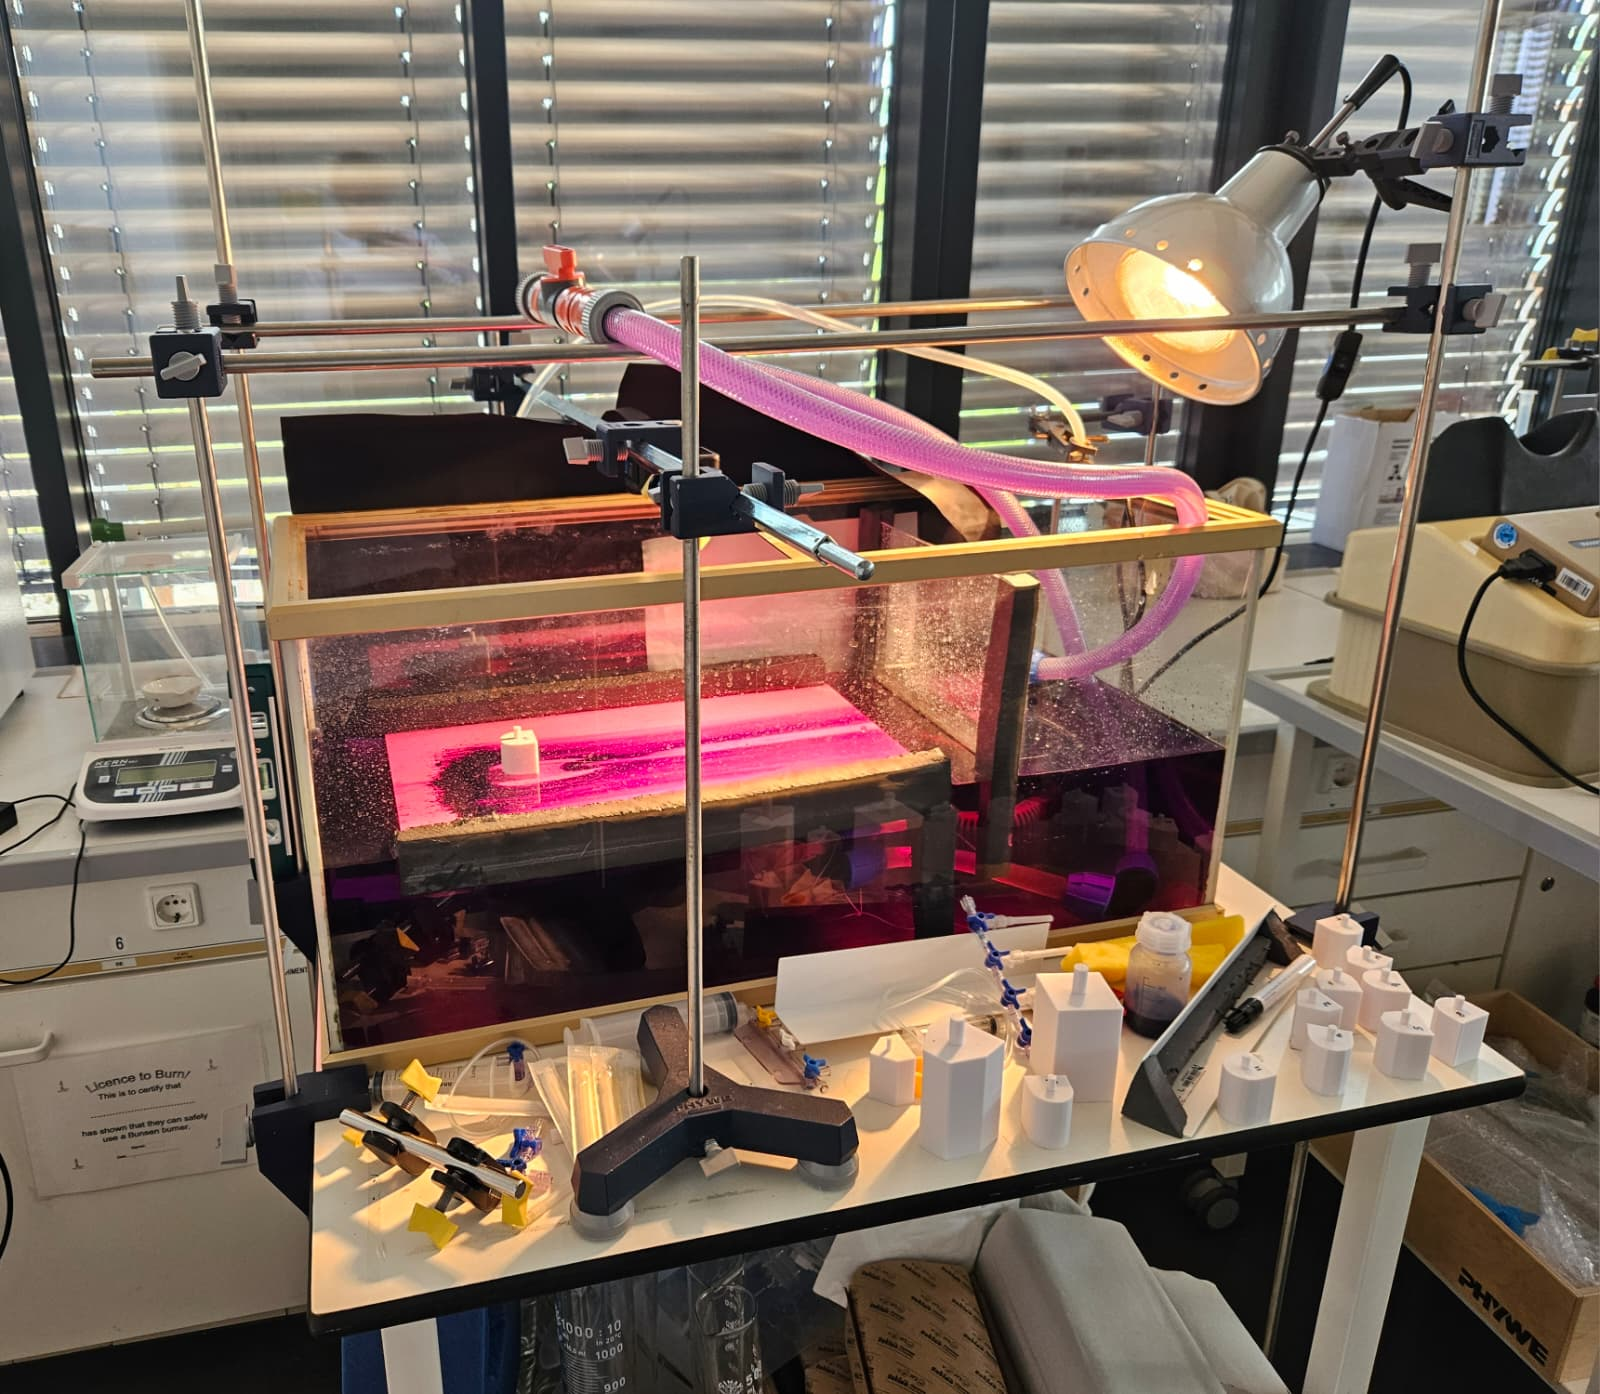
\includegraphics[width=\textwidth]{images/overallSetup1.jpg}};
		
		
		%Right
		\draw[->, line width=3pt, color=red] (6.5, 4.5) -- (4.2, 4.2);
		\node[fill=white, anchor=west] at (6.6, 4.5) {Lamp};
		
		\draw[->, line width=3pt, color=red] (6.5, 3.25) -- (2, 3.3);
		\node[fill=white, anchor=west, align=left] at (6.6, 3.25) {Hose (water \\ supply)};
		
		\draw[->, line width=3pt, color=red] (6.5, 2) -- (2.9, 2.5);
		\node[fill=white, anchor=west] at (6.6, 2) {Clamp};
		
		\draw[->, line width=3pt, color=red] (6.5, 0) -- (3.9, 1);
		\node[fill=white, anchor=west] at (6.6, 0) {Piping \diameter $0.017\,m$};
		
		\draw[->, line width=3pt, color=red] (6.5, -1) -- (2, -0.2);
		\node[fill=white, anchor=west, align=left] at (6.6, -1) {Separation wall (2)};
		
		\draw[->, line width=3pt, color=red] (6.5, -2) -- (1.35, -1.6);
		\node[fill=white, anchor=west, align=left] at (6.6, -2) {Separation wall (1)};
		
		\draw[->, line width=3pt, color=red] (6.5, -4) -- (0.1, -1.8);
		\node[fill=white, anchor=west, align=left] at (6.6, -4) {Sponge diffuser};
		
		
		%Left
		\draw[->, line width=3pt, color=red] (-6.5, -2) -- (-5, 0);
		\node[fill=white, anchor=east, align=left] at (-6.6, -2) {Aquarium};
		
	\end{tikzpicture}
	\caption{The setup for the practical investigation (angle 1)}
	\label{fig:overallSetup1}
\end{figure}

\begin{figure}[H]
	\centering
	\begin{tikzpicture}
		\path[use as bounding box] (-8, -7.5) rectangle (10, 7);
		
		\node[inner sep=0pt] (img) at (0,0) {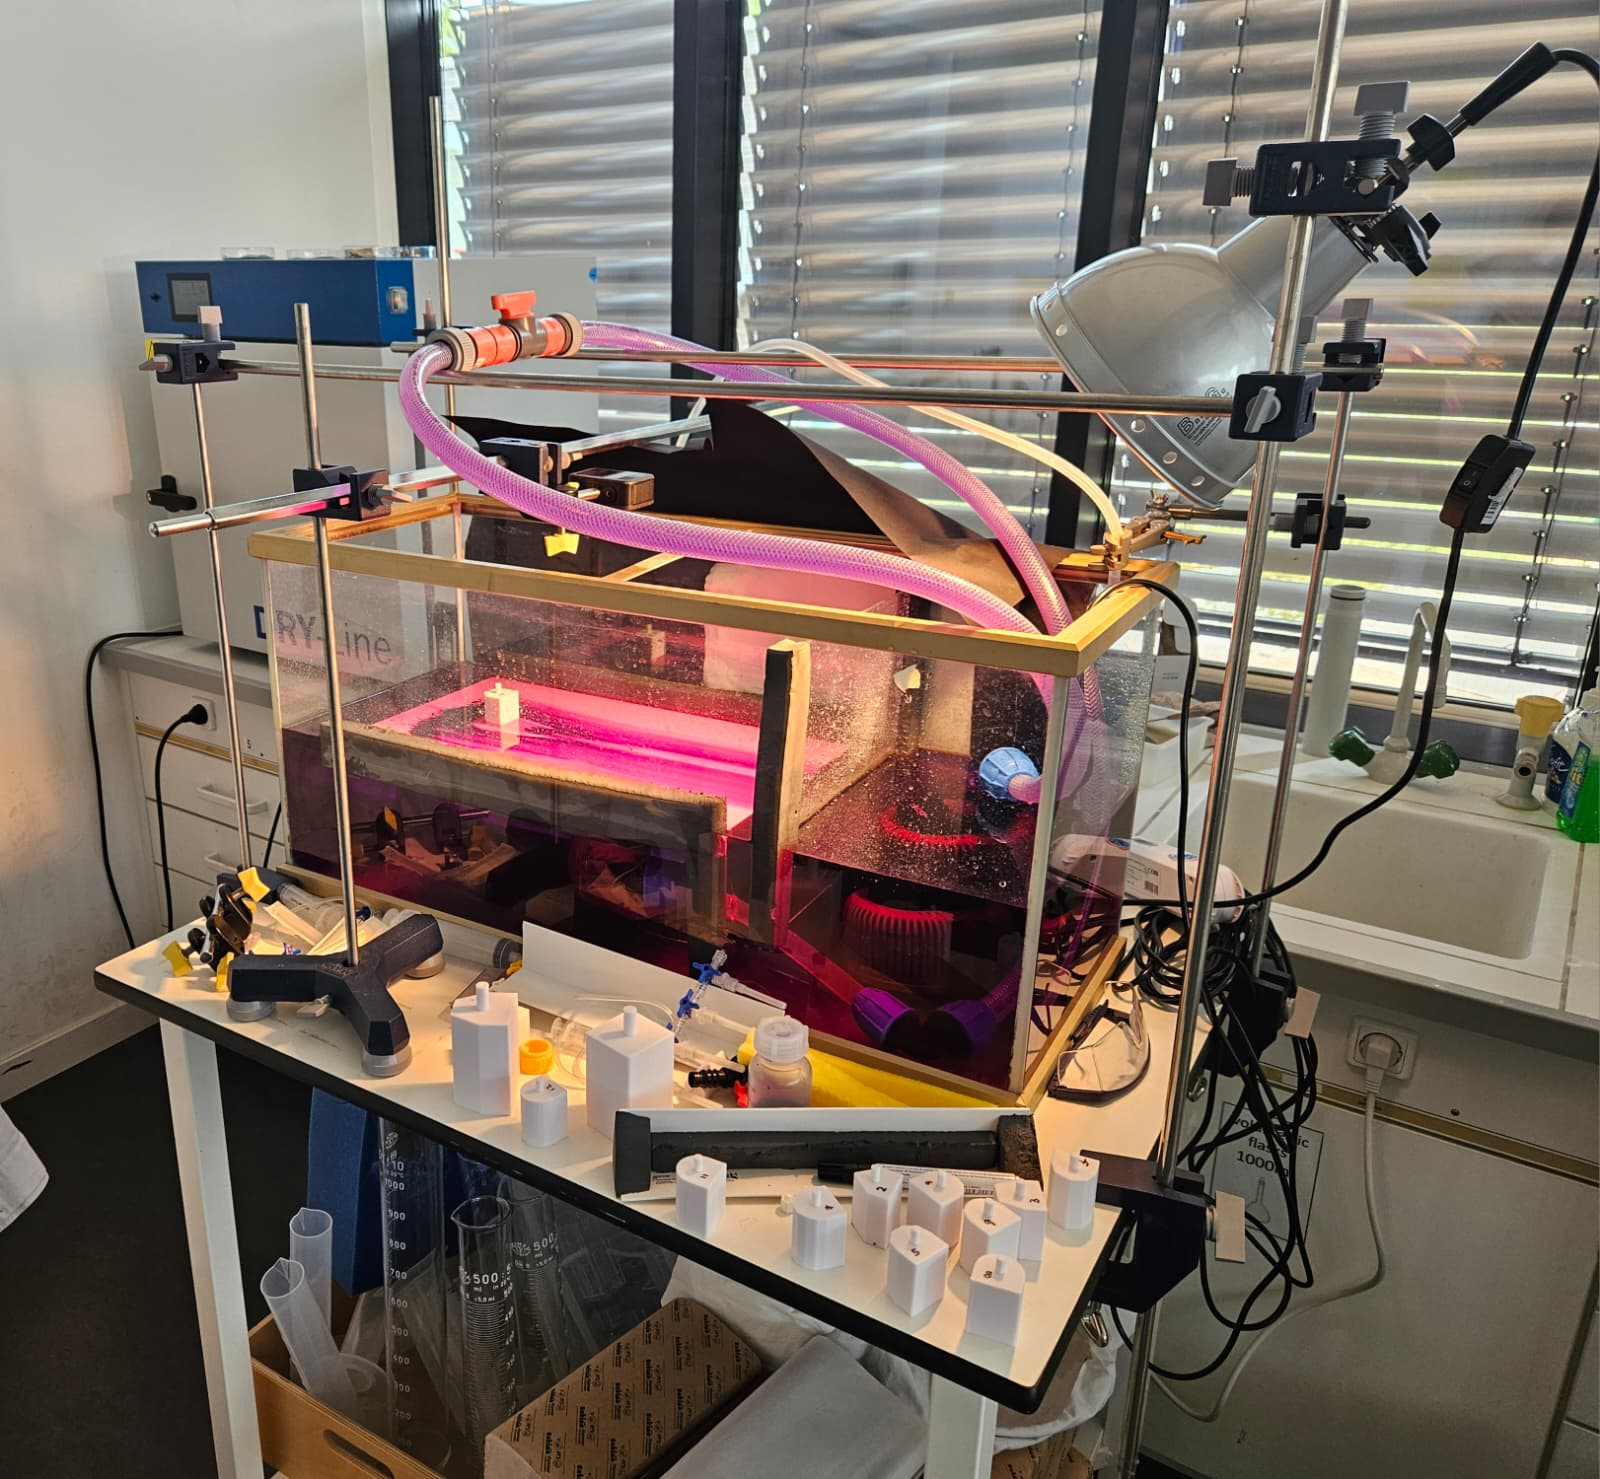
\includegraphics[width=\textwidth]{images/overallSetup2.jpg}};
		
		%Right
		\draw[->, line width=3pt, color=red] (6.5, 2) -- (4.9, 3.3);
		\node[fill=white, anchor=west] at (6.6, 2) {Boss};
		
		\draw[->, line width=3pt, color=red] (6.5, 0) -- (4.4, 1);
		\node[fill=white, anchor=west] at (6.6, 0) {Metal rod};
		
		\draw[->, line width=3pt, color=red] (6.5, -1) -- (0.4, 0);
		\node[fill=white, anchor=west] at (6.6, -1) {Clear acrylic glass};
		
		\draw[->, line width=3pt, color=red] (6.5, -2) -- (1.3, -2);
		\node[fill=white, anchor=west, align=left] at (6.6, -2) {75W Water pump};
		
		\draw[->, line width=3pt, color=red] (6.5, -3) -- (1.5, -3);
		\node[fill=white, anchor=west, align=left] at (6.6, -3) {Pipe corner piece};
		
		\draw[->, line width=3pt, color=red] (6.5, -4) -- (3.8, -4.6);
		\node[fill=white, anchor=west, align=left] at (6.6, -4) {Screw clamp};
		
		
		%Left
		\draw[->, line width=3pt, color=red] (-6.5, -4) -- (-5, -2.5);
		\node[fill=white, anchor=east, align=left] at (-6.6, -4) {Table stand};
		
		\draw[->, line width=3pt, color=red] (-6.5, 1) -- (-2, 2.5);
		\node[fill=white, anchor=east, align=left] at (-6.6, 1) {GoPro};
		
		\draw[->, line width=3pt, color=red] (-6.5, 4) -- (-3, 4);
		\node[fill=white, anchor=east, align=left] at (-6.6, 4) {Regulation value};
		
	\end{tikzpicture}
	\caption{The setup for the practical investigation (angle 2)}
	\label{fig:overallSetup2}
\end{figure}

\begin{figure}[H]
	\centering
	\begin{tikzpicture}
		\node[inner sep=0pt] at (0,0) {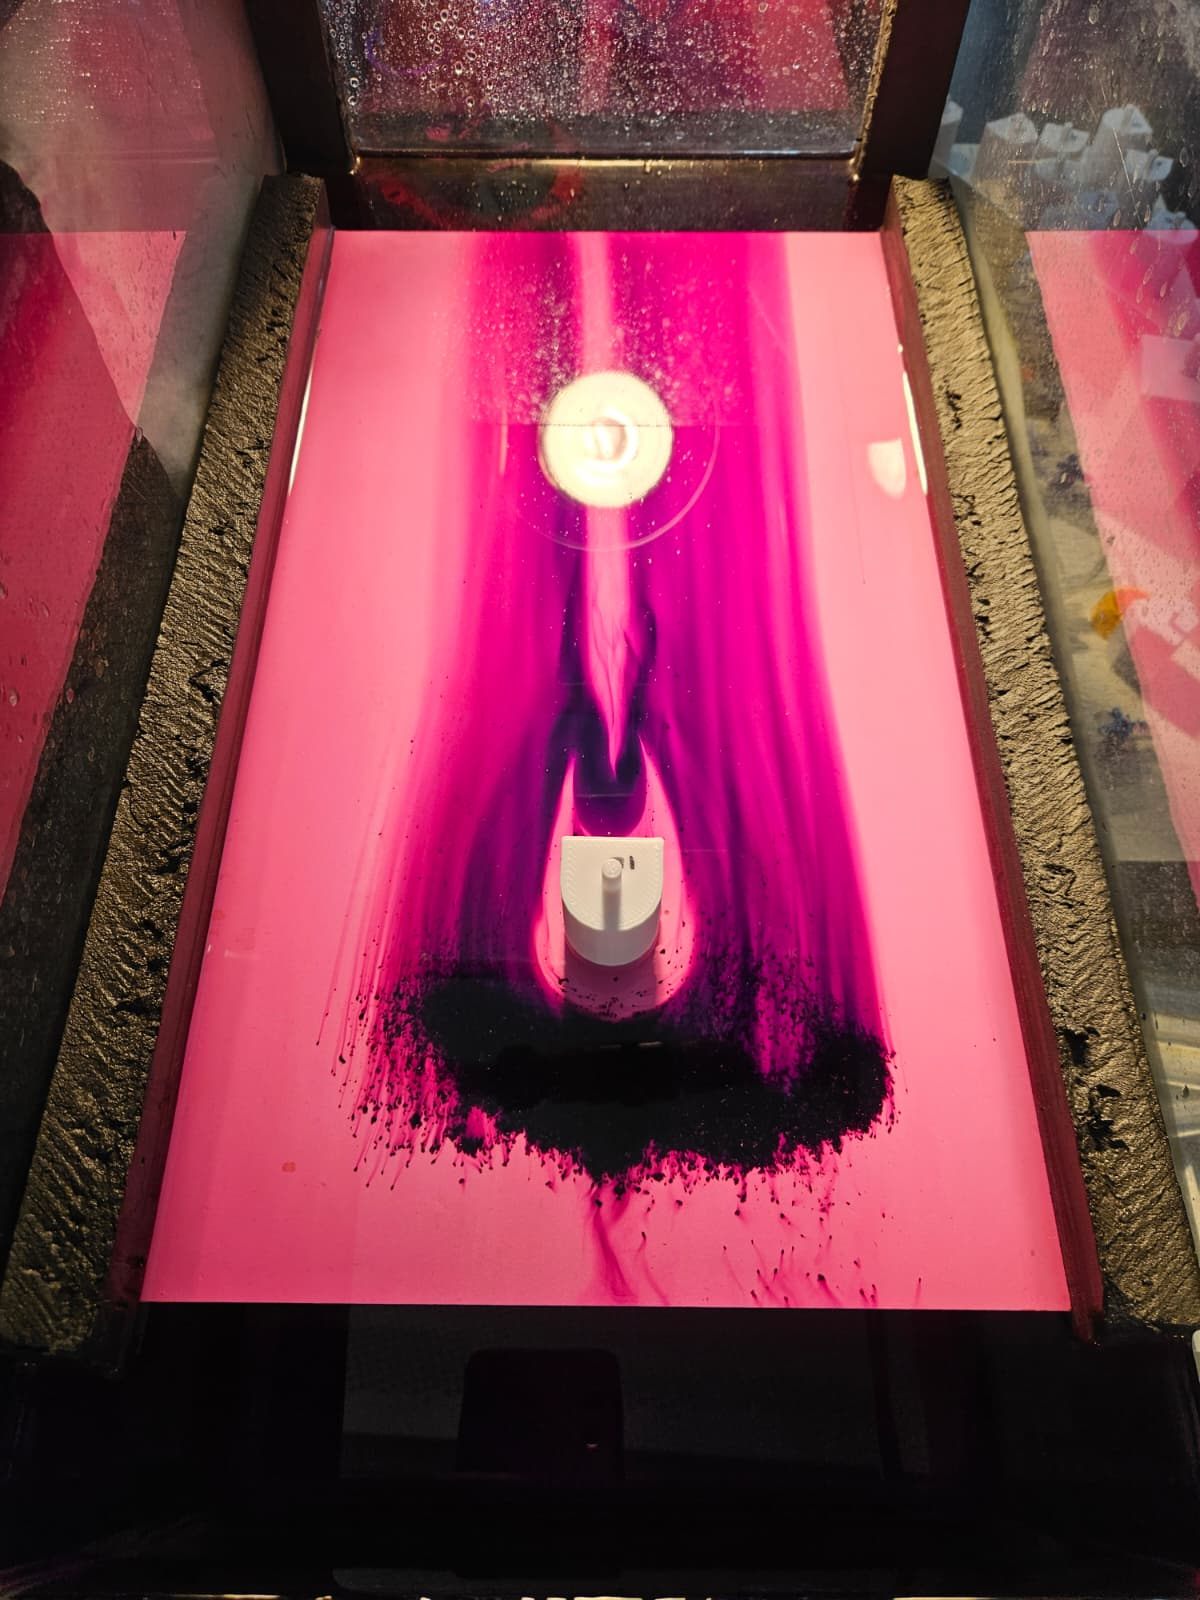
\includegraphics[width=\textwidth]{images/shapeInTank.jpg}};
		
		%Left
		\draw[->, line width=3pt, color=red] (6.5, 4.5) -- (5, 4.2);
		\node[fill=white, anchor=west, align=left] at (6.6, 4.5) {Thermal insulation \\ foam};
		
		\draw[->, line width=3pt, color=red] (6.5, 2) -- (3.7, 2.5);
		\node[fill=white, anchor=west] at (6.6, 2) {White acrylic glass};
		
		\draw[->, line width=3pt, color=red] (6.5, -1) -- (0.9, -2);
		\node[fill=white, anchor=west, align=left] at (6.6, -1) {Reference Mark};
		
		\draw[->, line width=3pt, color=red] (6.5, -4) -- (0.8, -4);
		\node[fill=white, anchor=west, align=left] at (6.6, -4) {Potassium \\ permanganate \\ crystals};
		
		
	\end{tikzpicture}
	\caption{A bluff body positioned in the flow tank with potassium permanganate crystals spread in front of it}
	\label{fig:shapeInTank}
\end{figure}

\begin{figure}[H]
	\centering
	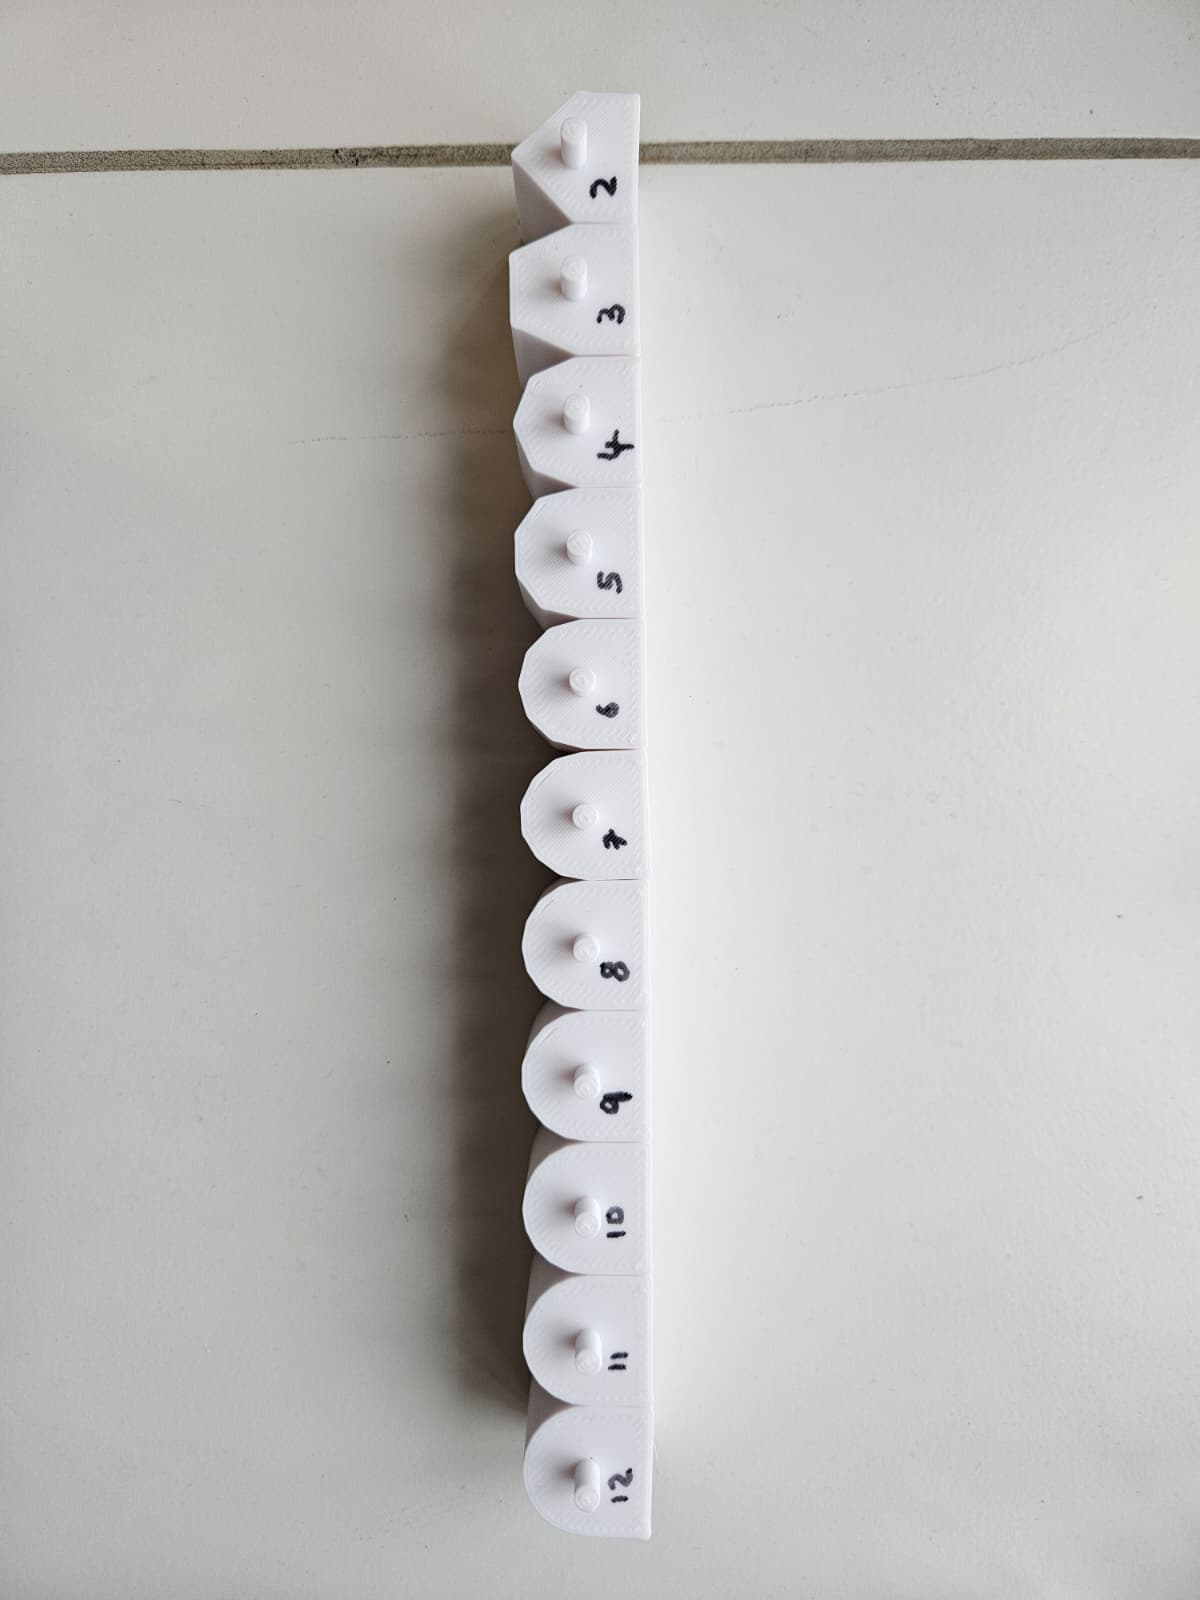
\includegraphics[width=\textwidth]{images/shapes.jpg}
	\caption{The 3D-printed bluff bodies. The numbers correspond to the number of inlet-facing sides}
	\label{fig:shapes}
\end{figure}

\newpage

Inspired by the flow tank built by Harvard University’s Science Demonstrations Center \parencite{noauthor_vortex_nodate}, the practical part of this EE was conducted in a self-built flow tank. A water pump created a flow over a horizontal plate by moving water from one side of separation wall (1) to the other. Separation wall (2), which did not reach the bottom of the tank, forced the flow of the horizontal wall towards the pump. The aquarium was filled with water so that it reached $0.01\,m$ above the horizontal plate. The regulation valve was used to decrease the flow velocity while the sponge diffuser ensured a uniform distribution of flow \textemdash\ in an attempt to achieve laminar flow. Both a lamp and the addition of potassium permanganate crystals in front of the shape were used in order to better visualize the water flow. The thermal insulation foam ensured watertightness between the aquarium wall and the inside components. 

The bluff bodies were 3D printed with an overall length $\ell$ of $0.02\,m$ \textemdash\ giving each shape a characteristic length $L$ of $0.02\,m$ \textemdash\ and a height of $0.04\,m$. Pre-tests showed that this overall length proved to be the optimal balance between the size of the bluff bodies and adequate identification of produced vortices, in an attempt to achieve a Reynolds number of $100$. Reference marks on the horizontal plate ensured the shape was positioned consistently each trial. A GoPro recording in 120 FPS was mounted parallel to the horizontal plate, ensuring a continuous recording of the entire horizontal plate. The outer scaffolding provided support for the lamp, the GoPro and the water supply hose. 

The flow velocity for the subsequent calculation of the Reynolds number was measured using a basic time-distance method, wherein a float was introduced and the time taken to travel the length of the horizontal plate was measured via a digital stopwatch. This was repeated ten times and an average was taken.

\subsection{Determining the vortex shedding frequency}
The inverse relationship given by Equation \eqref{eq:fAndT} in section \Cref{sec:fAndT} will be used to determine the vortex shedding frequency. By measuring the time interval between the formation of two consecutive vertices on one side of the bluff body, one can find the time period and therefore the frequency of vortex shedding. To obtain an accurate vortex shedding frequency, the determination of the time period was completed after periodic vortex shedding was achieved, omitting the initial startup phase in which the flow developed. A Fast Fourier Transform approach was not chosen due to the lack of sufficient runtime during the trials on either investigation and the absence of multiple different frequencies of vortex shedding \parencites[10--11]{shi2025vortex}[12]{xu_experimental_2025}.

\subsubsection{Theoretical Investigation}
\label{sec:theoreticalMethod}
The simulation was run five times for each bluff body. It was found that each iteration of a bluff body yielded the same results, therefore only the first run of each bluff body was considered. By graphing fluctuations of the lift coefficient \textemdash\ as can be seen in \Cref{sec:C_LvsTime} \textemdash\ one can calculate the time period of vortex shedding by identifying the time taken between two consecutive peaks or troughs. This determination was done for each peak and trough using python, removing the first second to omit the startup phase. An average time period was then calculated and the vortex shedding frequency was found. ParaView was used to visualize the simulation.

\subsubsection{Practical Investigation}
The bluff bodies were placed into the flow tank at the position of the reference marks. Wearing gloves and goggles, minimal amounts of potassium permanganate were placed in front of them using a spatula \textemdash\ as shown in \Cref{fig:shapeInTank}. Once the flow fully developed, it was recorded for one minute each time. This minimized the number of water replacements \textemdash\ due to dissolving potassium permanganate turning the water purple \textemdash\ while ensuring that one could take multiple measurements of the time period. The water was reused for four shapes before the aquarium was emptied using a hand pump \textemdash\ disposing the solution in a properly assigned waste tank \textemdash\ and was refilled with fresh water. 

The time period of vortex shedding was found via visual inspection of the GoPro footage and using a digital stop watch. It was repeated ten times for each bluff body. An average was subsequently calculated and the vortex shedding frequency was determined.
